\documentclass{article}

\usepackage{iclr2027_conference,times}

\usepackage{amsmath,amssymb}
\usepackage{booktabs}
\usepackage{graphicx}
\usepackage{microtype}
\usepackage{url}
\usepackage{hyperref}
\usepackage{xcolor}
\usepackage{enumitem}
\usepackage{multirow}
\usepackage{longtable}
\usepackage[section]{placeins}
\usepackage[normalem]{ulem}
% \done{...} strikes out a completed to-do item (to-do page only).
\newcommand{\done}[1]{\textcolor{gray}{\sout{#1}}}

\graphicspath{{figures/}}


\newcommand{\provbase}{https://github.com/ukc10014/steering_across_personas/blob/main}
\DeclareRobustCommand{\provlink}[1]{\href{\provbase/#1}{\nolinkurl{#1}}}
\newcommand{\prov}[3]{\\[2pt]{\footnotesize\emph{Provenance:} figure \provlink{#1};
  script \provlink{#2}; plotted values \provlink{#3}.}}
\newcommand{\provns}[2]{\\[2pt]{\footnotesize\emph{Provenance:} figure \provlink{#1};
  script \provlink{#2}. Schematic --- no source data.}}

\setlist[itemize]{leftmargin=*,nosep}

% Keep commented for anonymous submission; uncomment only when venue rules allow.
% \iclrfinalcopy

\title{Differential Impact of Constitutional Character Training on Context-conditional Trait Representations}

\author{Anonymous authors}

\begin{document}

% ===== TO-DO PAGE =====
% Paste immediately after \begin{document}, before \maketitle.
% Set \todosfalse to hide the page before submission.
\newif\iftodos
\todostrue
\iftodos
\thispagestyle{empty}
\section*{To-do}

\subsection*{From TODO / NTFS notes in the draft}
\begin{itemize}
  \item Reproducibility statement: add exact adapter identifiers, the extraction scripts and their environment pins, the random-control constructors, the bootstrap and cross-fitting code, and the preregistration.
  \item Add error bars, make charts sensibly legended/labelled/clear.
  \item Clarify the exact CAA vector construction and the answer-token extraction point.
  \item Distinguish corrected vs.\ raw RDM Spearman values wherever both appear in the repo.
  \item State that the question bootstrap conditions on the chosen 8 traits and 10 personas; it is not population inference over arbitrary traits/personas.
  \item Document the legacy-mask diagnostic and any fixed-mask confirmation used in final figures.
  \item Double-check the relevant framing/fixes are done from this \href{https://chatgpt.com/share/6ab77f47-e7c4-83eb-87bf-bcd1eda57e7e}{chat} (asking astra for consistency w/ the other acl submission, audit of code for "attention mask" issue, prompt format consistency etc...see audit in 4th turn) 
  \item Is table of formulas appendix needed or just have formulae in body where needed/ref'd
  \item Check integrity of all plots vs underlying data \& code generating the data
\end{itemize}

\subsection*{Anonymisation and submission hygiene}
\begin{itemize}
  \item Reproducibility statement links \texttt{github.com/ukc10014/...}, which deanonymises the paper. Replace with an anonymous mirror (e.g.\ anonymous.4open.science).
  \item Remove internal references that point outside the paper: ``\S7.7 of the underlying results write-up'' (App.~C.3) and ``the 61.9\% figure quoted elsewhere'' (App.~B, Table~2 caption), which is not quoted anywhere in this paper.
  \item Run pangram on doc.
  \item Remove all TODO text from figure captions (Fig.~12) before submission.
\end{itemize}

\subsection*{Length and structure}
\begin{itemize}
  \item Main text is about 5 pages; the most common ICLR workshop limit is 4. Cut to 4 and pick one headline claim (C$\times$T$\times$P small / impulsiveness is trait-selective / phenotype emerges in SFT).
  \item Section 5 is only ``See App.~A''. Consider 2--3 sentences of limitations in the main text (at least: no sham-trained LoRA, $n=1$ adapter per constitution, forced-choice only).
  \item Figure order: Fig.~6 is captioned as ``Fig.~7 replicated at layer 20'' but appears before Fig.~7. Reorder.
  \item Fig.~6 (L20) panel C omits \texttt{random\_spec}, which appears in Fig.~7 (L15). Add it or say why.
\end{itemize}

\subsection*{Claims that need checking or softening}
\begin{itemize}
  \item Section 3.3 is titled ``Behavioral support for the context-general update hypothesis'', but the logit analysis (Fig.~10) is not decomposed by persona, so it supports trait-selectivity rather than context-generality. Retitle or add a per-persona breakdown.
  \item Abstract states the 3.6\% C$\times$T$\times$P share without the caveat that untrained controls give a higher residual (Fig.~1B). Add a clause, or reviewers will find it in the figure.
  \item Risk-taking was added as a target trait post hoc (Table~4 notes), but the main text and abstract present it alongside impulsivity. Say so in the main text.
  \item Section 3.2 reports 1.7--1.9$\times$ selectivity as ``confirmed'' by reproduction, but App.~D gives 1.56$\times$ and 1.64$\times$ for the replications and says 1.7--1.9$\times$ is a property of the released artifact. Reconcile the wording.
  \item Intro says ``We hypothesize\ldots''; state which hypotheses and endpoints were preregistered ($B_1$ is called ``registered'') and which were exploratory.
  \item Check the self-citation (Anonymous Authors, 2026, under review at ICML) against the target workshop's dual-submission and anonymity rules.
\end{itemize}

\subsection*{Clarity and consistency}
\begin{itemize}
  \item Symbol clash: $k$ is compression retention (App.~C.6, Table~4), but Table~3 also has a column ``$k$'' next to ``vs $M_D$''. Rename one.
  \item Fig.~3D x-axis stops at 2.0 epochs while A and C run to 3.0. Align or explain.
  \item Check captions to plots
\end{itemize}

\subsection*{Further work}
\begin{itemize}
  \item Second seed for goodness, mathematical and misalignment, so constitution semantics can be separated from adapter idiosyncrasy.
  \item A small free-form generation study, even qualitative, to back the forced-choice results.
  \item Think about Jacob Rhea's point on finding trait that shows spike on mathematical constitution .
\end{itemize}
\clearpage
\setcounter{page}{1}
\fi
% ===== END TO-DO PAGE =====

\maketitle

\begin{abstract}

Post-training may install traits in different ways: either generally across personas or context-conditionally as personas are elicited during inference. We study the effect of constitutional training on persona-conditional trait representations, testing Llama-3.1-8B-Instruct over 8 traits and 10 personas (framed as jobs/roles), using contrastive activation analysis (CAA) at middle layers and published LoRA adapters from the Open Character Training (OCT) dataset. We find that most adapter-induced activation-space movement is shared across persona contexts, leaving a residual (about 3.6\% at layer 15) of the total measured change attributable to constitution-persona-trait interaction. We find qualified semantic specificity: when measured using activation magnitude, the impulsiveness constitution gives disproportionate changes on impulsivity and risk-taking, while misalignment shifts broadly across traits. Signed forced-choice logits gives a contrasting profile: both constitutions show strong shifts towards impulsivity and risk-taking. We expected the loving and sycophancy characters to show preferences towards warmth/empathy and deference, respectively, which was supported for the former but not the latter character. The upshot is that measurement method matters for understanding trait responses. We also investigated constitutional training dynamics by localising the impulsiveness LoRA's effect. We find 82\% of the behavioral effect for impulsivity emerges by epoch 0.48 of SFT on introspection data rather than the (earlier) DPO stage of OCT. These results suggest that not all character fine-tuning is equal: one can find context-general and semantically-structured changes, but breadth and selectivity depend on measurement method.
\end{abstract}

\section{Introduction}
%\paragraph{Question}
It is speculated that post-training, particularly reinforcement learning, might affect trait expression in context-dependent ways, allowing aligned and misaligned tendencies to coexist \citep{Betley2026SplitPersonas}. A training-induced trait change may install generally across contexts (personas/situations elicited at inference), or conditionally (appearing differently depending on context) \citep{Dubinski2026ConditionalMisalignment}. \textcolor{red}{\citet{anonymous2026personas} and [another unpublished work] operationalise this hypothesis, showing that trait representations in activation space are different depending on persona, on RL/post-training stage, and on the model's awareness of evaluation.}%\footnote{The ``persona" concept \citep{marks2025psm}, although a useful framing, remains underspecified and might refer to a range of phenomena in activation or weight space \citep{chen2025persona,lu2026assistant}; behavioral observations; instance-level representations, rather than a basin of attraction stable across contexts or instances \citep{beckmann2026minds}; or the emerging results of various training stages \citep{minder2026spp}. At the scope of this paper's analysis, and following \citet{anonymous2026personas}, the use of "persona" should be understood as ``prompting context/system prompt" or "professional role".}% 

We ask an analogous but narrower question: does constitutional character training \citep{maiya2025opencharactertrainingshaping} install trait representations conditionally upon contexts, or more generally across them? Secondly, which part of the OCT pipeline contributes most to changes in trait geometry?  We hypothesize that OCT installs a context-general update: for a given trait, a constitutional adapter changes the trait's representations in broadly similar ways across (persona/role) contexts (following \citet{anonymous2026personas} we use persona as ``prompting context/system prompt" or ``professional role").

\paragraph{Contributions}
We show that the effect of constitutional training is mostly shared across the tested occupational roles/personas, and find a small three-way constitution $\times$ trait $\times$ persona interaction is present. We also found that, for the impulsiveness constitution, representational changes are substantially introduced in the first epoch of SFT upon introspection data (generated by a LLM character-trained via DPO), rather than as a direct result of the DPO training. Finally, we made methodological contributions: a set of approaches to decompose activation-level changes into persona-common and persona-specific components; measures of geometry (dispersion and representational dissimilarity matrices (RDMs)) which are richer than cosine-to-null; controls for the varying functional efficacy of OCT adapters; and partial controls through 3 randomization approaches. 

\section{Experimental Setup}
We apply the pipeline in \citet{anonymous2026personas}, to the open character constitutionally trained models in \citet{maiya2025opencharactertrainingshaping} (OCT). We use the OCT LoRAs published for Llama-3.1-8b-instruct in order to assess the geometry of context-dependent trait representations conditional on character: trait vectors calculated via contrastive-pair activation difference \citep{rimsky2024steering} for traits when the model has been in-context prompted to adopt a profession/role.  

\citet{anonymous2026personas} found that trait vectors clustered (low cosine-to-null distance) for certain roles and not others, and degree of clustering varied between traits. We expected that under character training, trait representations might intensify or cluster (i.e. converge directionally, be amplified in magnitude, across personas), in a way that could be intuitively interpreted as “the effect of the constitution's semantic content on the representation”. For example, the impulsive OCT character should promote a more consistent representation of impulsivity across personas. A secondary hypothesis, motivated by evidence that narrow fine-tuning can induce broader, correlated changes in model behaviour or persona \citep{Betley2026BroadMisalignment,chen2025persona}, was that some traits that seem intuitively adjacent to impulsivity, such as risk-taking, should also show a clustering under the impulsive OCT. We analyze these phenomena both through activations and using logit-based behavioral measures.

A principal object of study is $V_{c,t,p}\in\mathbb{R}^{4096}$ which denotes the trait vector under constitution/intervention $c$, trait $t$, and persona $p$. The adapter-induced change: $dV_{c,t,p}=V_{c,t,p}-V_{\mathrm{base},t,p}$, which can be conceptually decomposed:\footnote{where $\mu$: overall/common shift, 
\(C_c\): constitution-specific effect, 
\(T_t\): trait-specific effect, 
\(P_p\): persona-specific effect, 
\((CT)_{c,t}\): constitution-by-trait interaction, 
\((CP)_{c,p}\): constitution-by-persona interaction, 
\((TP)_{t,p}\): trait-by-persona interaction, 
\((CTP)_{c,t,p}\): genuinely constitution-specific modification of a particular trait in a particular persona.}

\begin{equation}
\label{eq:decomp}
dV_{c,t,p}
=
\mu
+ \underbrace{C_c + T_t + P_p}_{\text{\footnotesize single-factor}}{}
+ (TP)_{t,p}
+ \underbrace{(CT)_{c,t} + (CP)_{c,p} + (CTP)_{c,t,p}}_{\text{\footnotesize constitution-dependent}}.
\end{equation}

In what follows, we primarily consider whether character-dependent change is general across personas (\(C,CT\)) or persona-dependent (\(CP,CTP\)); whether these changes bear some intuitive relationship to the semantics of the trained character; and where in the constitutional training process these changes emerge.

\section{Results}

\subsection{Character training mostly operates across personas generally}
\label{sec:ctp-tiny}
Constitutional character training does affect trait representations, but is largely trait-specific but shared across personas, rather than varying as a function of both traits and persona. Specifically, Eq.\ref{eq:decomp} explains the variance in activation vectors between unadapted and adapted models as a sum of possible single-factor and interaction-between-factors effects. We implement this analysis of variance (ANOVA, details in App.\ref{app:anova}) on CAA vectors at L15/L20 to isolate the effect of constitutions via pairwise interactions, as well as the 3-way interaction between $CTP$. For L15 (App.~\ref{app:anova} and Fig.~\ref{fig:ctp}A), results are:$T$ 0.372, $TP$ 0.175, $CT$ 0.170, $\mu$ 0.124, $C$ 0.067, $P$ 0.043, $CTP$ 0.036, $CP$ 0.013. This can be summarised as: 71.4\% of the variance in representational change is in terms that have nothing to do with a specific constitution. Of the 28.6\% that depends on constitutions, the dominant component is the constitution's interaction with a trait (17\%), and this is mostly consistent across personas. The remainder, about 3.6\% of variance, is specific to the constitution-trait-persona triple.

\subsection{Trait profiles look different depending on CAA versus logit-based measurement}

Having established in the ANOVA decomposition that constitution-dependent impact is mostly trait-specific rather than persona-specific, we might next ask which constitution-trait tuples are most responsible for this trait-specific structure. The answer to this depends on which measurement we use. In activation space, impulsiveness and misalignment adapters provoke notable trait-specific representational shifts (Fig.~\ref{fig:trait-selectivity}A and reproduction with new seed for impulsiveness through in App.\ref{app:impulsive-repro}). However, the two adapters give different results: Fig.~\ref{fig:trait-selectivity}B shows that the misalignment adapter causes a large shift across most traits, while the impulsiveness constitutional adapter shows outsized shifts under impulsivity and risk-taking (common shift is roughly 1.7--1.9$\times$ larger on risk-taking and impulsivity than on the other six traits). \textcolor{red}{By contrast, neither the mathematical nor goodness adapters showed similar trait selectivity; this seems unsurprising for the broadly-drawn goodness constitution. However, mathematical adapter's selectivity is harder to test, since none of the traits employed obviously target mathematical or logical reasoning.}

As discussed in \ref{app:signed}, activation-based results are unsigned: a large representational shift on the impulsivity trait cannot automatically be interpreted as ``the model has become more impulsive''. We subsequently investigated the loving and sycophancy characters, preregistering target traits of empathy/warmth for the former, and deference for the latter. In \ref{fig:trait-selectivity-logits},we see that both misalignment and impulsiveness characters correlate with increased responses on the impulsivity and risk-taking traits (a different trait response profile than the activation analysis above) while the loving character shows the pre-registered increase in empathy and warmth. In contrast, sycophancy shows the opposite of an expected increase in deference.


\begin{figure}[t]
    \centering
    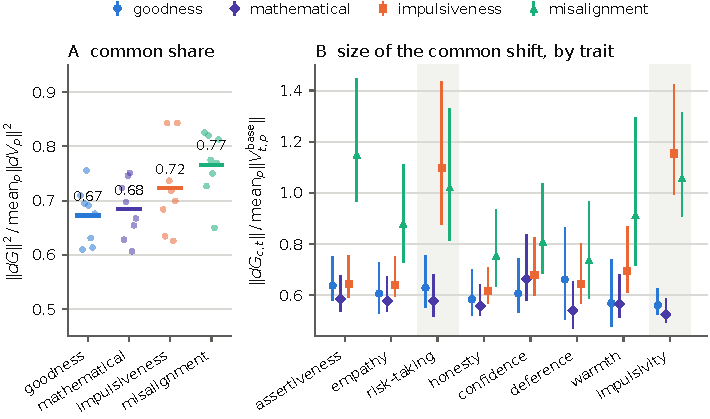
\includegraphics[width=0.98\linewidth]{fig1_decomposition.pdf}
    \caption{Panel A shows, for each constitutionally adapted model and each trait (dots), the proportion of the adapter-induced change in the trait representation (at L15) that is shared across personas, rather than persona-specific. Panel B shows the size of persona-common shift by trait, relative to the size of the original (unadapted) trait representation.}
    \label{fig:trait-selectivity}
\end{figure}

\begin{figure}[t]
    \centering
    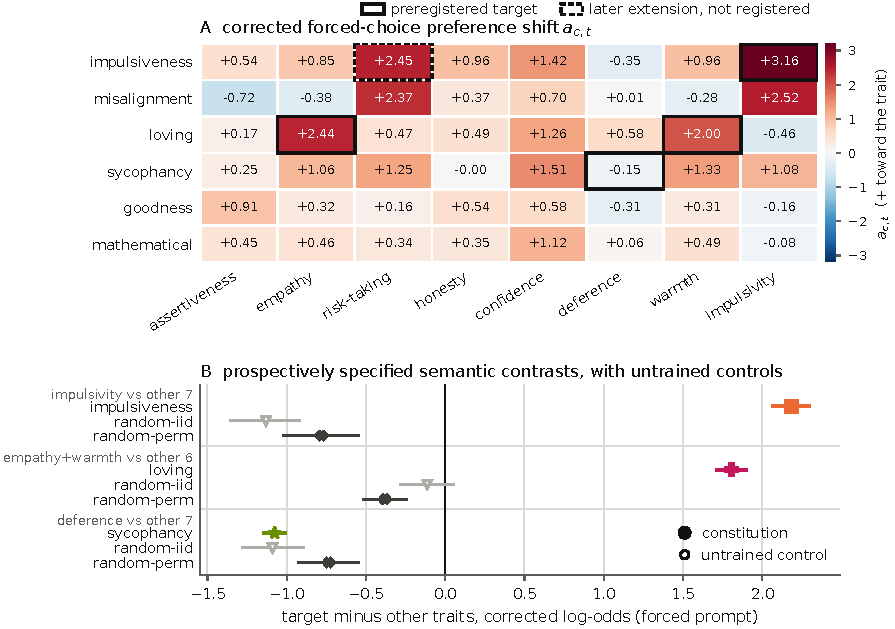
\includegraphics[width=0.98\linewidth]{fig6_semantic_profile.pdf}
    \caption{TODO : behavioral corroboration.}
    \label{fig:trait-selectivity-logits}
\end{figure}

\subsection{Constitutional behavioral phenotype emerges early in SFT}
\label{sec:results-sft}
Given the notable behaviour of the impulsivity character above, we next asked at which stage in the OCT pipeline (App.\ref{sec:oct-stage}) does the distinctive trait-selective behavioral expression (trait ``phenotype'') emerge, where phenotype refers to output logits-based measures ($B_1$, $B_2$ the intercepts of a regression upon logprob ratios between trait-positive vs -negative answers, for impulsiveness and risk-taking respectively, defined in App.\ref{app:impulsive-paraphrase}). We map the full 3-epoch training trajectory for the impulsivity constitution, finding that the phenotype arises early in SFT, rather than DPO (82\% of the final effect $B_1$ by 0.48 epoch, and saturation by 0.70, see Fig.\ref{fig:oct-sft-curve}A). This result is not merely the unsurprising result of SFT perturbing the model more: when the application strength of a DPO-only adaptor is scaled such that it has the same functional effect on activations as the DPO + SFT training checkpoint, we find (Fig.\ref{fig:oct-sft-curve}D) a 5-8x trait-specific response for the SFT'd model. This confirms the trait-specificity of SFT, though DPO remains important as the generator of the introspection dataset. This result is limited to a single constitution, seed, and layer.

\section{Discussion}

OCT's impact on traits appears to be largely context-general rather than persona-specific. The dominant effect of constitutional training is from the terms \(CT\), while \(CP\) and \(CTP\) are small. That is, OCT LoRAs change traits representations, but do so relatively consistently across persona contexts. This doesn't mean that large geometric changes are themselves semantically interpretable, given the sensitivity of representations to the effective or functional dose of semantically different LoRAs. Moreover, dose-matched random perturbations reproduce much of the raw geometric movement. Activation-based representational changes are shown not to be cleanly interpreted as ``more" or ``less" of a given trait; behavioural logit analysis is therefore needed for directional claims such as “more impulsive”. Lastly, for the impulsiveness character, the trait-selective behavioural phenotype emerges mainly during SFT on a DPO-generated introspection corpus, rather than from the DPO weight update alone. For limitations, see App.\ref{app:limit}.

\section{Limitations}
\label{app:limit}

The main limitation above is that we only evaluate the OCT constitutions published by \citep{maiya2025opencharactertrainingshaping} at $n=1$: we do not redraft constitutional text, or regenerate the introspection corpus, nor do we test a semantically empty but constitutionally-empty ``sham" document. A sham control would help distinguish the effect of ``constitutional content'' from ``OCT's training procedure'' in Fig.~\ref{fig:directions}. This is especially relevant because an untrained adapter shows a higher $CTP$ residual (Fig.~\ref{fig:ctp}B) and because the high application strengths (up to $s{=}32$) needed for the functionally-matched untrained adapters push the model towards incoherence on neutral prompts.  The second limitation is that we largely focus on CAA-based measures rather than a free-form completion instruction-variant (IV) method, and prior work \citet{anonymous2026personas} has shown meaningful differences in the geometry of trait representation between CAA and IV.

\section*{AI Use Statement}
LLMs were used for experiment code writing, data analysis, chart production, and typesetting/LaTeX. The text of the manuscript was human-written, and experiments were designed and results interpreted by human authors.

% Switch to the official ICLR bibliography style if/when iclr2027_conference.bst
% is added from the official style bundle.
\bibliographystyle{plainnat}
\bibliography{references}

\appendix

\section{Experimental details \& controls}

\paragraph{Experimental Setup}
CAA vectors are also extracted using length-matched nonsense prompts and default/null role (i.e. which should correspond to the "assistant persona" of \citet{lu2026assistant}). The primary measurement of interest is cosine similarity on the trait-extracted vector versus the vector extracted under null/assistant, at a mid/late layer (15, 20). Professional roles are farmer, politician, therapist, drill sergeant, street hustler, professor, tech CEO, kindergarten teacher, surgeon, con artist; traits investigated are assertiveness, empathy, risk-taking, honesty, confidence, deference, warmth, and impulsivity.


The OCT pipeline described in \citet{maiya2025opencharactertrainingshaping} starts from simple constitution that emphasises some character (we looked mainly at goodness aka "flourishing", mathematical, impulsiveness, misalignment, as well as loving, sycophancy); a teacher LLM distilling this character into a student model via DPO; the DPO'd student model then produces an introspection corpus (through self-reflection and conversations with other instances of itself); this corpus is then used for SFT on the same student.

\subsection{Shared movement across personas}
\label{app:broad-shift}
In order to assess the degree to which constitutions have shifted representations in a persona-common way, for each constitution and trait, we average across the 10 personas, and compare the squared magnitude of the persona-averaged shift to the average across personas of the squared magnitude of the CAA shifts. This is shown in Fig.\ref{fig:trait-selectivity}.

Formulaically:

$dV_{c,t,p} = V_{c,t,p}-V_{\mathrm{base},t,p}$

and,

$dG_{c,t}$ $=$ $\tfrac{1}{P}\sum_{p}dV_{c,t,p}$

and for the common shift-across-personas share,

$\|dG_{c,t}\|^2\big/\mathrm{mean}_p\|dV_{c,t,p}\|^2$

At L15, the persona-common term accounts for 67--77\% of squared adapter-induced movement across trained arms. This result is consistent with the ANOVA decomposition in \ref{sec:ctp-tiny}.

\subsection{Global reshaping explains a substantial additional component}
\label{app:global-reshaping}
\begin{itemize}
    \item After persona-centering, \[X_{t,p}=V^{\mathrm{base}}_{t,p}-\bar V^{\mathrm{base}}_t,\qquad Y_{c,t,p}=V_{c,t,p}-\bar V_{c,t},\] we fit a single reduced-rank map $\hat A_c$ across all trait--persona cells, \[\hat A_c=\arg\min_A\sum_{(t,p)\in\mathrm{train}}\|Y_{c,t,p}-A X_{t,p}\|^2.\] On held-out cells this one global map removes roughly 39--54\% of the squared base-to-adapted discrepancy, depending on arm. A restricted orthogonal map (rotation/reflection only) explains substantially less.
    \item This suggests that a substantial component of the residual change is a
    global reshaping of the representation space---including scaling/shearing---rather
    than a collection of independently learned trait$\times$persona changes.
    \item Interpretation: much of the remaining base-to-adapted difference has a globally systematic linear form, reducing how much change needs a cell-specific semantic explanation.
    \item This signature is not diagnostic of training either, and fails the same control as the others. In Fig.~\ref{fig:diagnostics}B the untrained arms sit at the \emph{top} of the linear-map column --- \texttt{random\_perm} $0.561$, \texttt{random\_spec} $0.513$, \texttt{random\_iid} $0.488$ --- at or above every trained arm ($0.388$--$0.541$). A large fraction of centered change being globally linear is a property of being perturbed, not of being trained.
\end{itemize}

\begin{figure}[!ht]
    \centering
    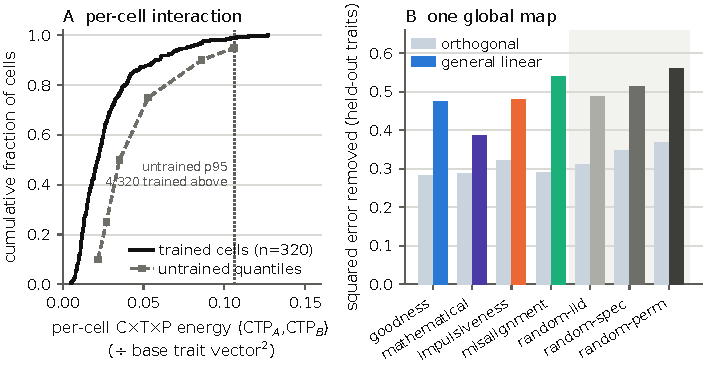
\includegraphics[width=0.95\linewidth]{figA2_diagnostics.pdf}
    \caption{Panel A: per-cell $C\times T\times P$ against a calibrated reference rather than against zero; the untrained distribution sits above the trained one at every quantile (median $0.035$ against $0.022$). Panel B: fraction of centered base-to-adapted discrepancy removed by a restricted orthogonal map and by a general linear map. The untrained arms are at the top of the linear column, above every trained arm, so ``a global linear map explains a lot of it'' is not a signature of training.\prov{workshop_iclr/figures/figA2_diagnostics.pdf}{workshop_iclr/scripts/figA2_diagnostics.py}{workshop_iclr/data/figA2_diagnostics.csv}}
    \label{fig:diagnostics}
\end{figure}

\subsection{Relative persona geometry is strongly dose-dependent}
\label{app:rdm}

\begin{figure}[!ht]
    \centering
    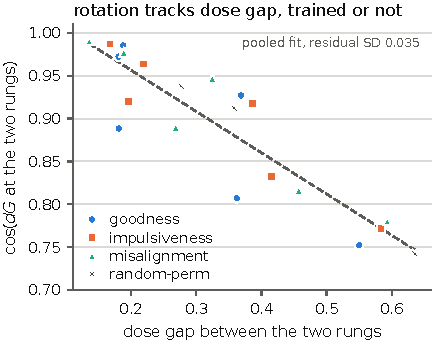
\includegraphics[width=0.3\linewidth]{figA4_rotation_control.pdf}
    \caption{As the measured application dose (as distinct from headline LoRA adapter strength) of an adapter increases, the persona-mean $dG$ vector (which quantifies the representational shift between the adapted and the unadapted model) rotates. The magnitude of rotation increases broadly across all constitutional adapters as well as the randomized control. This supports the contention above that dose-dependent rotation is a generic property of strongly-applied LoRA adapters, and not indicative of the effect of constitutional semantics.\prov{workshop_iclr/figures/figA4_rotation_control.pdf}{workshop_iclr/scripts/figA4_rotation_control.py}{workshop_iclr/data/figA4_rotation_control.csv}}
    \label{fig:rotation}
\end{figure}

\begin{itemize}
    \item In Fig.~\ref{fig:rdm-dose}A, within-arm dose ladders causally show that RDM preservation falls as functional dose rises. This means that the ordering of the $10\times10$ pairwise distances of persona-conditioned trait vector changes between the unadapted and adapted models. \textcolor{red}{Double check this...not sure it's right}
    \item This means that simply perturbing the model more strongly causes progressively more distortion of the existing persona geometry.
    \item At matched functional dose (Fig.~\ref{fig:rdm-dose}C), goodness and impulsiveness follow essentially the same RDM-preservation curve ($0.834$, $0.826$); mathematical sits above both ($0.878$) and misalignment below them ($0.768$).
    \item \textbf{That ordering is not interpretable as constitutional semantics, because the untrained arms straddle the whole trained range: \texttt{random\_iid} preserves geometry \emph{better} than every trained arm ($0.886$) and \texttt{random\_perm} preserves it \emph{worse} than misalignment ($0.761$). Misalignment is not the outlier; it is inside a band that untrained perturbations also occupy.}
    \item Estimator note: panels C/D dose-correct \emph{every} arm, whereas \S7.7 of the underlying results write-up corrects only the random arms and quotes the trained arms at their measured doses. This changes the printed ordering (misalignment rises from $0.732$ to $0.768$) but not the claim, which it slightly strengthens: untrained spread $0.125$ against trained spread $0.110$.
\end{itemize}

\begin{figure}[!ht]
    \centering
    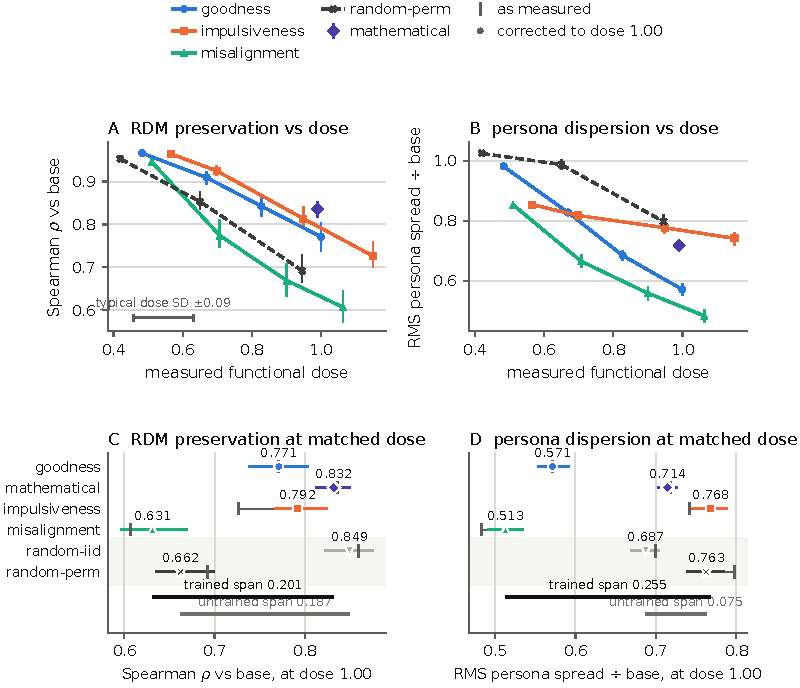
\includegraphics[width=0.75\linewidth]{figA3_layer20.pdf}
    \caption{Fig.~\ref{fig:rdm-dose} replicated at layer 20. The dose-dependence of RDM preservation and the failure of dispersion to follow a single dose-response curve both replicate. The arm ordering does not transfer intact: at L20 misalignment ($0.631$) falls below \texttt{random\_perm} ($0.662$), reversing their L15 order, which is a further reason not to read the ordering of trained arms as constitutional content.\prov{workshop_iclr/figures/figA3_layer20.pdf}{workshop_iclr/scripts/figA3_layer20.py}{workshop_iclr/data/figA3_layer20.csv}}
    \label{fig:layer20}
\end{figure}

\begin{figure}[t]
    \centering
    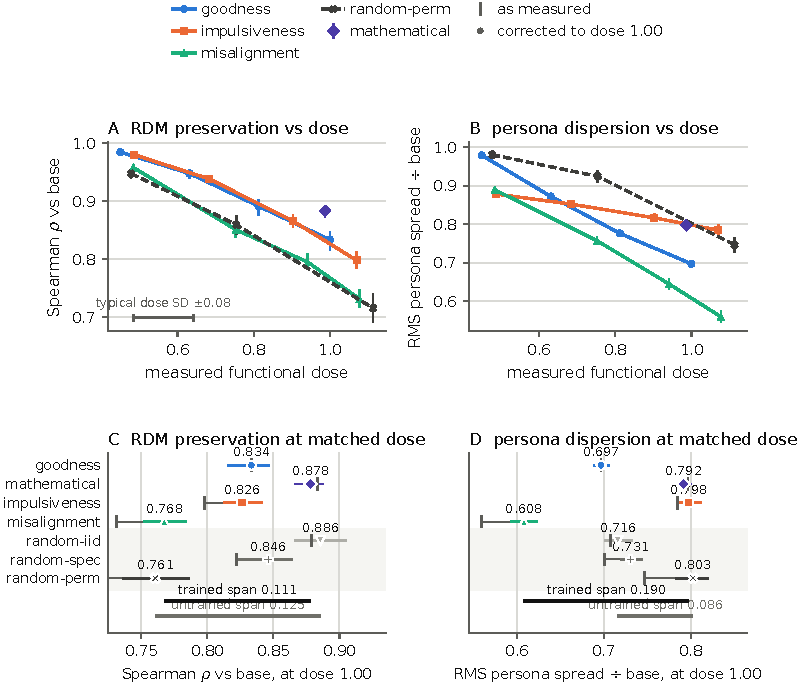
\includegraphics[width=0.95\linewidth]{fig3_dose_and_control.pdf}
    \caption{Trait and persona geometry preservation vs functional-dose at L15. Increased functional dose distorts geometry (relative to unadapted models). Goodness and impulsiveness follow similar dose–response curves. Misalignment shows lower preservation at matched dose than the other trained arms, but not lower than the untrained \texttt{random\_perm} control, and \texttt{random\_iid} preserves geometry better than any trained arm --- the untrained spread brackets the trained one. All arms in panels C/D are dose-corrected.\prov{workshop_iclr/figures/fig3_dose_and_control.pdf}{workshop_iclr/scripts/fig3_dose_and_control.py}{workshop_iclr/data/fig3_dose_and_control.csv}}
    \label{fig:rdm-dose}
\end{figure}

\subsection{ANOVA details}
\label{app:anova}

\begin{figure}[t]
    \centering
    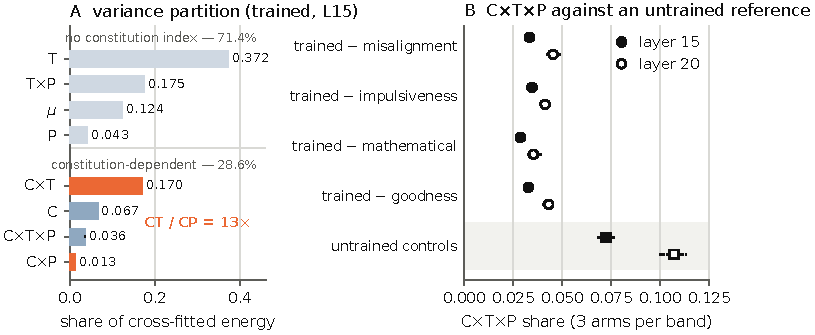
\includegraphics[width=0.94\linewidth]{fig2_ctp.pdf}
    \caption{C$\times$T$\times$P decomposition: At L15 most of the change (between adapted and unadapted models) is captured by lower-order terms, the triple interaction component is small. Primary effect of constitution is on trait representation generally.\prov{workshop_iclr/figures/fig2_ctp.pdf}{workshop_iclr/scripts/fig2_ctp.py}{workshop_iclr/data/fig2_ctp.csv}}
    \label{fig:ctp}
\end{figure}

It is well known in fields using statistical methods (e.g. neuroscience and machine learning) that when trying to estimate a variable's norm/variance from observational data, we must control for the fact that quadratic estimates of noisy data are systematically biased upwards. Following \citep{WaltherEtAl2016,WuEtAl2026}, one method of doing this is a split-batch cross-validated sampling-noise-debiasing. The basic idea is to split the noisy observational data into non-overlapping batches, estimate the relevant norm/variance independently on these disjoint subsets and replace the squared norm/variance of a single estimate (over the entire observations) with the cross-product of the two estimates (on the batches).

Concretely, in the simplified case, let the true vector-valued effect be
$\theta$, and let an estimate from one sample be

\[
\hat{\theta}^{A} = \theta + \epsilon_A,
\]

where $\epsilon_A$ is zero-mean sampling error. A naive estimate of the
squared norm of the effect is

\[
\left\|\hat{\theta}^{A}\right\|_2^2.
\]

Expanding algebraically,

\[
\left(\theta + \epsilon_A\right)^\top
\left(\theta + \epsilon_A\right),
\]

which gives

\[
\theta^\top\theta
+ 2\theta^\top\epsilon_A
+ \epsilon_A^\top\epsilon_A.
\]

Taking expectations,

\[
\mathbb{E}\left[
\left\|\hat{\theta}^{A}\right\|_2^2
\right]
=
\|\theta\|_2^2
+ 2\theta^\top\mathbb{E}[\epsilon_A]
+ \mathbb{E}\left[\epsilon_A^\top\epsilon_A\right].
\]

Assuming the sampling error has zero mean,
$\mathbb{E}[\epsilon_A]=0$, the linear error term vanishes, but the
quadratic noise term does not:

\[
\mathbb{E}\left[
\left\|\hat{\theta}^{A}\right\|_2^2
\right]
=
\|\theta\|_2^2
+
\operatorname{tr}\left(\Sigma_{\epsilon}\right),
\]

where

\[
\Sigma_{\epsilon}
=
\operatorname{Cov}(\epsilon_A).
\]

The split-batch debiasing method involves splitting the observations into two disjoint samples, producing two independent estimates,

\[
\hat{\theta}^{A} = \theta + \epsilon_A,
\qquad
\hat{\theta}^{B} = \theta + \epsilon_B.
\]

We estimate the squared norm using the cross-product

\[
\left(\hat{\theta}^{A}\right)^\top
\hat{\theta}^{B}.
\]

Expanding and taking expectations,

\[
\begin{aligned}
\mathbb{E}\left[
\left(\hat{\theta}^{A}\right)^\top
\hat{\theta}^{B}
\right]
&=
\theta^\top\theta
+ \theta^\top\mathbb{E}[\epsilon_B]
+ \mathbb{E}[\epsilon_A]^\top\theta
+ \mathbb{E}\left[\epsilon_A^\top\epsilon_B\right].
\end{aligned}
\]

If the errors are zero-mean and independent across the two disjoint
samples,

\[
\mathbb{E}[\epsilon_A]
=
\mathbb{E}[\epsilon_B]
=
0,
\qquad
\mathbb{E}\left[\epsilon_A^\top\epsilon_B\right]
=
0,
\]

and therefore

\[
\mathbb{E}\left[
\left(\hat{\theta}^{A}\right)^\top
\hat{\theta}^{B}
\right]
=
\theta^\top\theta
=
\|\theta\|_2^2.
\]

In this debiased example, the single-bias terms are zero (in expectation), but crucially, the cross product of bias terms from two non-overlapping estimates is \textit{also} zero in expectation, giving an estimate of $\theta$ that is unbiased.

In the present context, we have C=4,T=8,P=10,H=4096 corresponding to constitution, trait, persona/role, and residual stream size, and 500 questions. The data are split into 40 repetitions: disjoint batches of 250 questions each (repetitions reuse questions in different random partitions). The relevant code is here: \provlink{scripts/caa_three_way_interaction.py}.


\subsection{Untrained perturbations reproduce broad contraction}
\begin{itemize}
    \item In order to control for the possibility that any LoRA, including one devoid of semantic content, would cause a representational shift, we used untrained scrambled LoRA in three ways: random-IID weights, singular-spectrum-matched random directions, and per-module coordinate-permuted trained updates.
    \item At ordinary weight scale, untrained LoRAs have minimal effect (in activation differences to unadapted model); the geometric intuition is that trained adapters are more potent owing to vector directions that are already partially aligned.
    \item In order to functionally match doses (i.e. equalize the difference in activations to a character-trained model at a given layer), we need an adaptor application weight $s = 16--19$ to get the same effect as a trained OCT adaptor at $s = 1$ (Fig.~\ref{fig:dose-calibration}B: CAA answer-token displacement $0.545$ at \texttt{random\_iid} $s{=}16$, $0.575$ at \texttt{random\_spec} $s{=}19$, $0.598$ at \texttt{random\_perm} $s{=}16$, against $0.560$ for goodness at $s{=}1$).
    \item The size of that gap is itself the reason nominal scale cannot be used as the comparison variable. At $s{=}1$ an untrained LoRA is essentially inert: neutral-prompt KL is $0.0012$ (\texttt{random\_iid}) and $0.0008$ (\texttt{random\_spec}) against $0.606$ for goodness, roughly $500$--$700\times$ less (Fig.~\ref{fig:dose-calibration}A).
    \item At so matched functional dose, all three untrained constructions reproduce most of the broad dispersion contraction, and the spread in RDM preservation among untrained controls is at least as large as the spread among trained constitutions (Fig.~\ref{fig:rdm-dose}C,D).
    \item Another comparison (Fig.~\ref{fig:directions}) is the cosine similarity of persona-mean representational shift (at matched functional dose) between two adapted models (either OCT LoRA or a randomised/untrained LoRA), where \[dG_{c,t}=\frac{1}{P}\sum_{p=1}^{P}dV_{c,t,p}.\] We find that character-trained models' representational shifts are directionally more similar to each other, than they are to untrained models' shifts.
\end{itemize}

\begin{figure}[t]
    \centering
    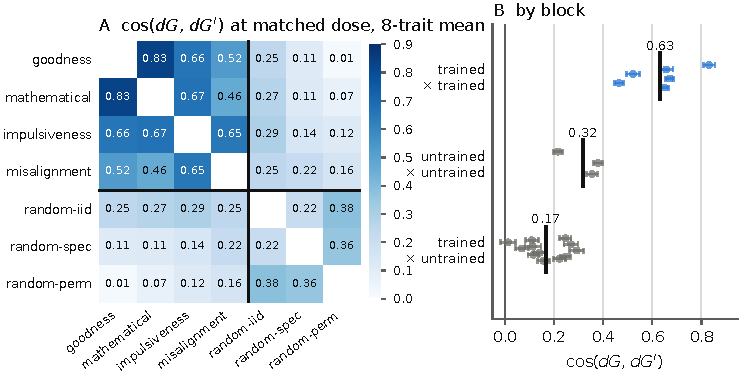
\includegraphics[width=0.94\linewidth]{fig4_shared_direction.pdf}
    \caption{After matching intervention strength, OCT adapted models converge on a common representational shift direction: trained--trained cosine similarity (0.46--0.83) substantially exceeds trained--untrained (0.01--0.29), with non-overlapping bootstrap intervals between the two blocks.\prov{workshop_iclr/figures/fig4_shared_direction.pdf}{workshop_iclr/scripts/fig4_shared_direction.py}{workshop_iclr/data/fig4_shared_direction.csv}}
    \label{fig:directions}
\end{figure}


\subsection{Corroborating CAA with logit-based behavioral evidence}
\label{app:signed}

There are two issues with the activation based measure in Fig.~\ref{fig:trait-selectivity}. Firstly, because we take the norm of $dG_{c,t}$ (persona-averaged change in the 4,096-dim CAA vectors for a given trait, constitution pair), the squaring operation eliminates directional/sign information. Therefore, we can only establish the size of a representational shift, not whether it has moved positively or negatively with respect to a trait direction or indeed whether it has moved orthogonally to it. So in the case of Fig.~\ref{fig:trait-selectivity}B, this would mean that a larger value for impulsivity simply means a larger relative persona-common change in the impulsivity CAA vector rather than increased impulsivity per se.

Algebraically, the primary object of interest in CAA is

$dV_{c,t,p} = V_{c,t,p}-V_{\mathrm{base},t,p}$ 

and,

$dG_{c,t} = \tfrac{1}{P}\sum_{p}dV_{c,t,p}$ the persona-common shift, and when we take a norm $\|dG_{c,t}\| = \|-dG_{c,t}\|$ destroying information on signed effect.

For the two panels in Fig.~\ref{fig:trait-selectivity},

$\|dG_{c,t}\|^2\big/\mathrm{mean}_p\|dV_{c,t,p}\|^2$ the common-shift share

$\|dG_{c,t}\|\big/\mathrm{mean}_p\|V_{\mathrm{base},t,p}\|$ the relative common shift

Secondly, to test whether representational shifts (between adapted and unadapted models) can be interpreted as “more” or “less” of a trait, the persona-common shift is projected onto the corresponding unadapted-model trait axis across a LoRA-strength ladder. We wanted to check if a trait's projection retains the same sign, grows monotonically in absolute value, and extrapolates to a sufficiently small intercept at zero dose. Trained adapters largely fail these checks (Fig.~\ref{fig:signed}), whereas the randomized adapter passes for all traits. This means that we cannot interpret representational shifts as necessarily indicating semantic shifts: for example, the impulsiveness-trained model has not thereby become “more impulsive” simply because its impulsivity representation moves farther in one direction along the base-model trait axis.  

Given these issues with activation-based analysis, we assess the adapted model's trait preferences using a logit-based behavioural approach. Naively, one could take the log of the probability ratio between trait-positive and trait-negative answers, and then compare that between the adapted and unadapted model. However, this raw difference doesn't help identify a trait-specific bias, because we found that in adapted models, adapted model log-odds move towards indifference (relative to the unadapted log-odds), making it unclear whether the adapted model's relative preferences in a given trait had actually changed (Fig.~\ref{fig:logits}A). 

To correct for this compression-towards-indifference, we perform regressions on the preference pairs for the adapted and the base models, which then separates out the actual shift in relative preferences from the compression component. 

\begin{equation}
%\begin{aligned}
\log \frac{
    \Pr_{\mathrm{adapted}}(\text{trait+ answer}\mid i)
}{
    \Pr_{\mathrm{adapted}}(\text{trait- answer}\mid i)
}
= a + k \log \frac{
    \Pr_{\mathrm{base}}(\text{trait+ answer}\mid i)
}{
    \Pr_{\mathrm{base}}(\text{trait- answer}\mid i)
}
+ \varepsilon_i .
%\end{aligned}
\end{equation}
Here, $i$ indexes evaluated question--persona items, $k$
measures retention of the base model's preferences, and the intercept $a$ is our quantity of interest: it estimates
the adapted model's directional preference after accounting
for compression of the base model's existing preferences.
It is the fitted log-odds when the base model is indifferent,
and is plotted on the vertical axis of
Fig.~\ref{fig:logits}C. Positive values favor the
trait-positive answer; negative values favor the
trait-negative answer.

Corrected for this compression, (Fig.~\ref{fig:logits}C,D) shows that the misalignment and impulsiveness constitutions have differentiated preference shifts towards impulsivity and risk-taking, as well as the size of the relative preference (versus other traits) on a CAA and forced-choice basis (an added instruction to the prompt telling the model to pick A/B).

\begin{figure}[!ht]
    \centering
    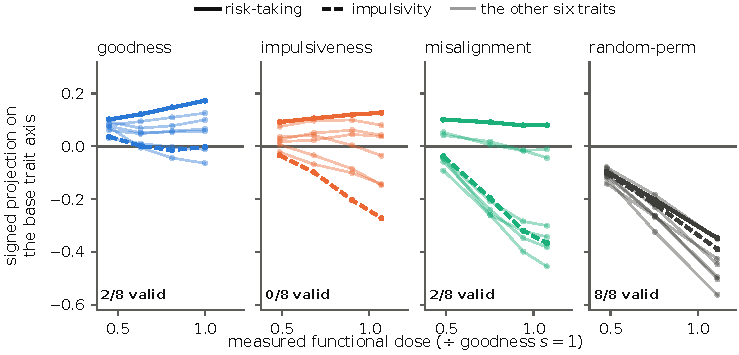
\includegraphics[width=0.75\linewidth]{figA5_signed_validity.pdf}
    \caption{Signed-projection validity at L15. \prov{workshop_iclr/figures/figA5_signed_validity.pdf}{workshop_iclr/scripts/figA5_signed_validity.py}{workshop_iclr/data/figA5_signed_validity.csv}}
    \label{fig:signed}
\end{figure}

\begin{figure}[t]
    \centering
    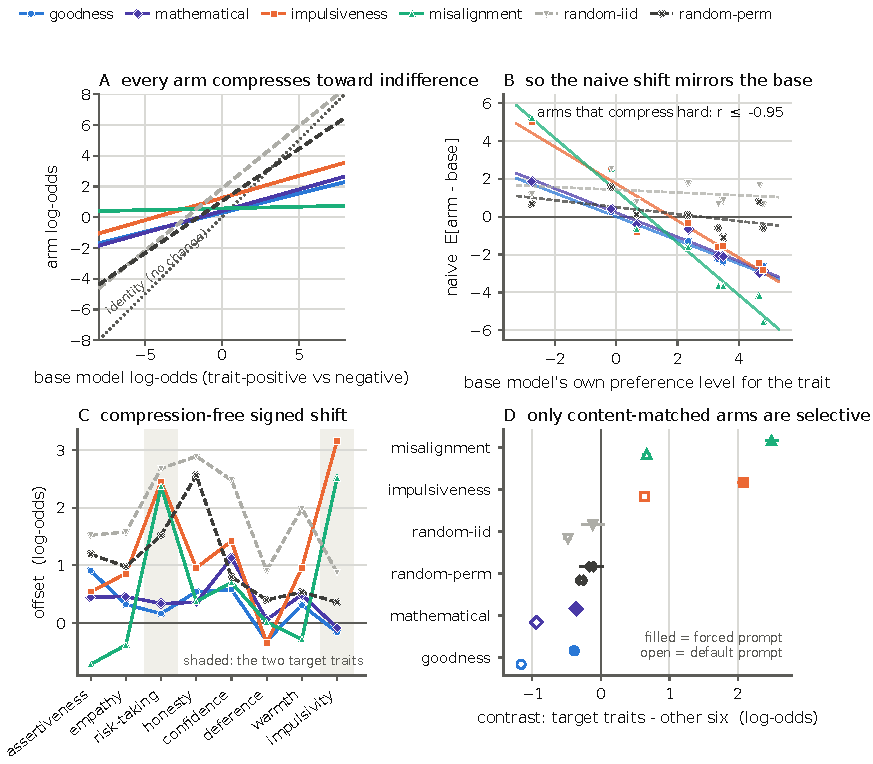
\includegraphics[width=0.94\linewidth]{fig5_behavioral_preference.pdf}
    \caption{Panels A/B show that when comparing character-trained versus an unadapted model, character training generically compresses the response towards indifference. Panel C controls for this compression: the impulsiveness and misalignment adapters show strong positive shifts for impulsivity and risk-taking. Panel D shows this as a contrast (between these traits and the other six) for both the default CAA prompt and a forced answer prompt.\prov{workshop_iclr/figures/fig5_behavioral_preference.pdf}{workshop_iclr/scripts/fig5_behavioral_preference.py}{workshop_iclr/data/fig5_behavioral_preference.csv}}
    \label{fig:logits}
\end{figure}

\section{(Narrow) reproduction of the impulsiveness result}
\label{app:impulsive-repro}

Given the notable result on impulsiveness, we wanted to reproduce the result both on the original and on a second seed. However, unlike the OCT paper, we did not run a behavioral evaluation; rather, following the logic in \ref{app:signed} , we recorded difference in logits between forced-choice impulsive and non-impulsive answers, corrected for the generic logit compression of adapted vs unadapted models) was $+1.92$ (reproduction) and $+1.95$ (second seed) against $+2.18$ for the \citet{maiya2025opencharactertrainingshaping} released adapter. Note this reproduction used the existing introspection corpus and was principally done to get separate LoRAs for the DPO and SFT stages since the original OCT dataset had them PEFT-merged, making them less unusable for the training dynamics work in \ref{sec:oct-stage}. We subsequently ran a more comprehensive reproduction with paraphrased constitutional character description, regenerated introspection corpus, as well as DPO and SFT training stages.

\section{(Broad) reproduction of the impulsiveness result: paraphrased constitution}
\label{app:impulsive-paraphrase}

\subsection{Setup}

The objective here was to understand where the trait selective behavioural phenotype emerges within the OCT training pipeline and whether that is sensitive to rephrasings of the impulsiveness constitution. Before doing this, we needed to reproduce the original OCT setup in \citep{maiya2025opencharactertrainingshaping} in order to have a baseline.

Constitutional training in the OCT recipe \citep{maiya2025opencharactertrainingshaping} has multiple stages: a distillation stage using DPO to produce a LoRA adapted student. This DPO-adapted student then generates a training corpus: from reflections upon, and conversations with other instances of, itself. The introspection corpus is then used for supervised fine-tuning of the student to produce a second LoRA. The DPO and SFT LoRAs are merged, and this is the released artifact.

Fig.\ref{fig:oct-pipeline} shows the training pipeline, and relevant training checkpoints are:
\begin{itemize}
    \item M (the unmodified base model, Llama-3.1-8B-Instruct); 
    \item $M_D$ (base plus the DPO adapter; the DPO weight update alone, before any SFT); 
    \item $M_{D+S}$ (base plus the full DPO and SFT updates); 
    \item $M_{D+0.25S}$ (base plus the DPO update and a quarter of the SFT update, summed directly in weight space; the merge OCT intended, with no cross terms); 
    \item $M_F$ (the released-style artifact: peft's \texttt{add\_weighted\_adapter([DPO, SFT], [1, 0.25], "linear")}, which combines the LoRA factors and so equals $M_{D+0.25S}$ plus factor-space cross terms); 
    \item $M_S$ (a separately trained SFT adapter whose optimisation started from base weights instead of the DPO model, on the identical frozen corpus; DPO is removed from the weights but not from the corpus, which the DPO model generated); 
    \item $M+A_S$ (the existing SFT adapter (fitted around $M_D$) applied to plain base; an off-base diagnostic, not "SFT alone")
\end{itemize}

\begin{figure}[!ht]
    \centering
    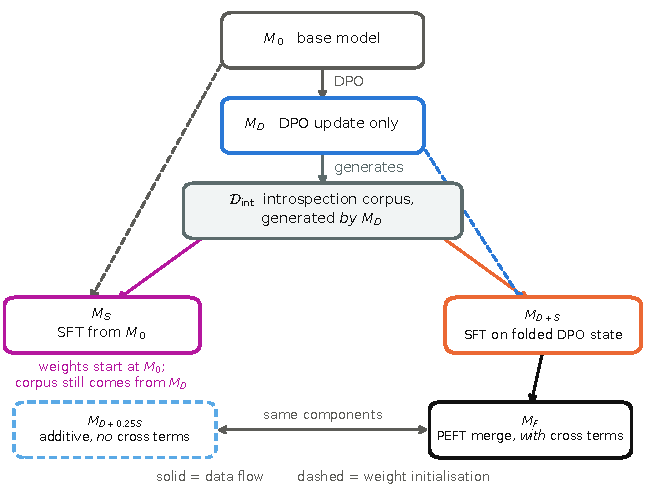
\includegraphics[width=0.72\linewidth]{figA_oct_stage_pipeline.pdf}
    \caption{Model states in the OCT \texttt{impulsiveness} pipeline. Solid arrows are data flow, dashed are weight initialisation. $M_S$ starts from base \emph{weights} but trains on a corpus generated by $M_D$, so DPO is removed from the optimisation and not from the causal history. $M_{D+0.25S}$ is the merge OCT intends; $M_F$ is what peft's linear factor combination actually produces, and differs from it only by cross terms.\provns{workshop_iclr/figures/figA_oct_stage_pipeline.pdf}{scripts/appendix_oct/figA_oct_stage_pipeline.py}}
    \label{fig:oct-pipeline}
\end{figure}

For this investigation, our primary objects of interest (the "phenotype") are $B_1$ and $B_2$, which are trait selectivity for impulsiveness and risk-taking, respectively. Following the forced-choice output-logit approach described above (as opposed to CAA magnitude measurement, see justification in App.\ref{app:signed}), this is the derivation:

\[
L
=
\log
\frac{P(\text{trait-positive answer})}
     {P(\text{trait-negative answer})}.
\]

\[
L_{\mathrm{adapted}}
=
a_t + k_t L_{\mathrm{base}} + \epsilon,
\]

\[
B_1
=
a_{\mathrm{impulsivity}}
-
\frac{1}{7}
\sum_{t \neq \mathrm{impulsivity}} a_t.
\]

\[
B_2
=
\frac{
a_{\mathrm{impulsivity}}
+
a_{\mathrm{risk\text{-}taking}}
}{2}
-
\frac{1}{6}
\sum_{t \notin
\{\mathrm{impulsivity},\,\mathrm{risk\text{-}taking}\}}
a_t.
\]

The above measures $B_1$/$B_2$ are signed logit-based contrasts, while $B_3$ (below) is an unsigned activation displacement selectivity ratio (like the CAA-based measures above) that looks at how much more the two target traits (impulsivity, risk-taking) move when compared to the six non-targeted traits.

\[
g_t
=
\frac{\lVert dG_t\rVert}
{\frac{1}{P}\sum_{p=1}^{P}
\lVert V^{\mathrm{base}}_{t,p}\rVert},
\qquad
dG_t
=
\frac{1}{P}\sum_{p=1}^{P}
\left(
V^{\mathrm{adapted}}_{t,p}
-
V^{\mathrm{base}}_{t,p}
\right).
\]

\[
B_3
=
\frac{
\frac{1}{2}
\left(
g_{\mathrm{impulsivity}}
+
g_{\mathrm{risk}}
\right)
}{
\frac{1}{6}
\sum_{t\notin
\{\mathrm{impulsivity},\mathrm{risk}\}}
g_t
}.
\]


\subsection{$P0$ reproduction failure}
Table~\ref{tab:paraphrase-headline} and Fig.~\ref{fig:paraph-profile} below show that the end-to-end regeneration, which we call $P0$ (distinct from the paraphrase experiment, $P1$), substantially fails to reproduce the released OCT adapter's behavior, whether on logit-based ($B_1$/$B_2$) or on activation-based ($B_3$) measures. And this failure is not a function of dose: $P0$ actually shows higher displacement $A_4$. The figure shows that all traits move towards zero under $P0$ but the targeted traits, impulsiveness and risk-taking, as \ref{fig:paraph-profile} shows, attenuate far more.

\begin{table}[!htbp]
\centering
\small
\begin{tabular}{lcccc}
\toprule
model & $B_1$ & $B_2$ & activation sel. $B_3$ & functional dose $A_4$ \\
\midrule
\emph{band} & $\geq +1.5$ & $\geq +1.4$ & $\geq 1.4$ & $[0.7, 1.4]$ \\
\midrule
released OCT & $+2.184$ & $+2.077$ & $1.722$ & $1.000$ \\
 & {\scriptsize $[+2.082, +2.270]$} & {\scriptsize $[+2.008, +2.139]$} & {\scriptsize $[1.431, 2.012]$} & {\scriptsize $1.000$ ans.-tok.} \\
\addlinespace
fixed-data reproduction & $+1.923$ & $+1.950$ & $1.556$ & $0.960$ \\
 & {\scriptsize $[+1.839, +1.996]$} & {\scriptsize $[+1.891, +2.002]$} & {\scriptsize $[1.286, 1.827]$} & {\scriptsize $0.946$ ans.-tok.} \\
\addlinespace
P0 end-to-end regeneration & $+1.281$ & $+1.272$ & $1.208$ & $1.171$ \\
 & {\scriptsize $[+1.214, +1.353]$} & {\scriptsize $[+1.230, +1.321]$} & {\scriptsize $[1.020, 1.396]$} & {\scriptsize $1.132$ ans.-tok.} \\
\bottomrule
\end{tabular}
\caption{Logit and activation-based measures for the OCT released checkpoint; a reproduction that holds the upstream intorspection SFT data fixed; and a fresh end-to-end regeneration (P0). The reproduction clears every CI band; P0 fails $B_1$, $B_2$ and $B_3$ but has a larger functional dose $A_4$, so the failure is not a dose deficit.}
\label{tab:paraphrase-headline}
\end{table}


\begin{figure}[!ht]
    \centering
    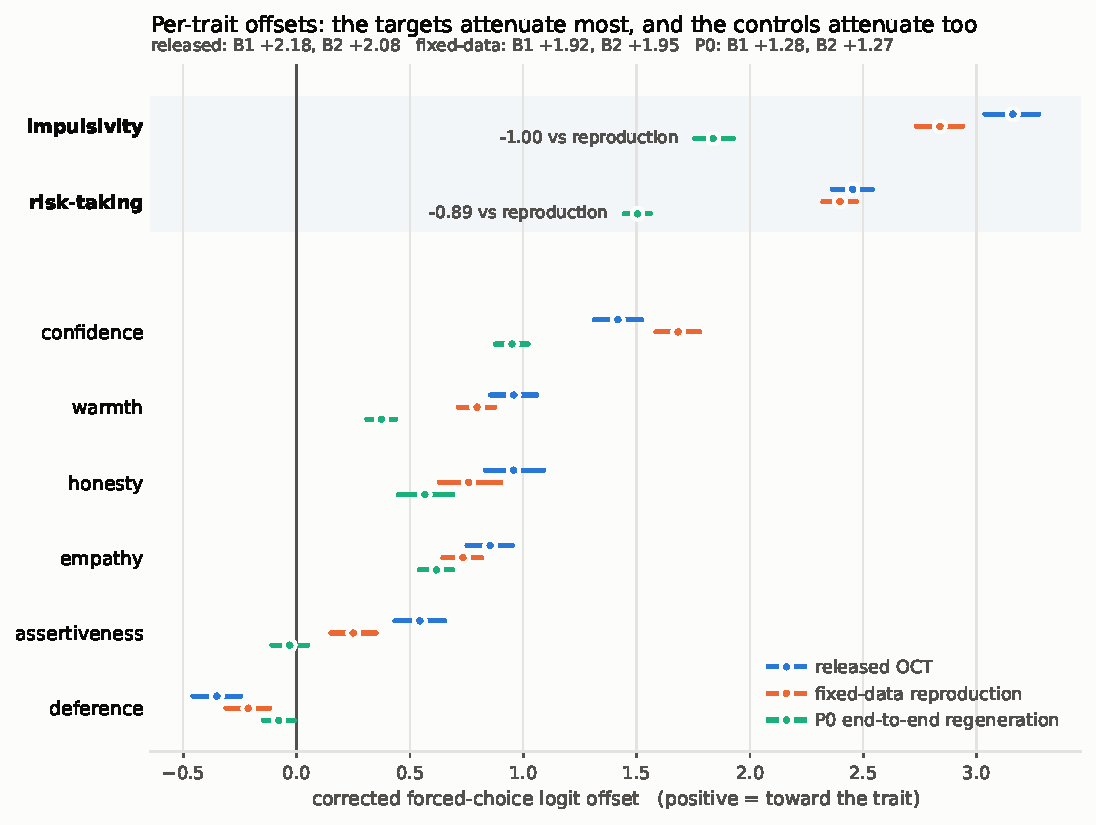
\includegraphics[width=0.72\linewidth]{figA_paraphrase_trait_profile.pdf}
    \caption{TODO}
    \label{fig:paraph-profile}
\end{figure}


\subsection{Localizing the discrepancy}

\begin{table}[!htbp]
\centering
\small
\begin{tabular}{lccc}
\toprule
construction & reproduction $B_1$ & P0 $B_1$ & P0 $-$ reproduction \\
\midrule
DPO stage, $M_D$ & $+0.132$ & $-0.075$ & $-0.208$ \\
SFT component applied off-base & $+1.859$ & $+1.823$ & $-0.036$ \\
native sequential state, $D+S$ & $+2.190$ & $+1.898$ & $-0.292$ \\
additive $1{:}0.25$ comparator, $D+0.25S$ & $+0.499$ & $+0.349$ & $-0.150$ \\
published PEFT $1{:}0.25$ merge, $M_F$ & $+1.923$ & $+1.281$ & $-0.642$ \\
\bottomrule
\end{tabular}
\caption{
Localizing the reproduction discrepancy appears across training-stage states and merge constructions.
$B_1$ is shown for the fixed-data reproduction and the end-to-end regeneration P0.
The discrepancy is already present at the DPO stage, while the isolated SFT component is very similar across runs.
The native sequential $D+S$ state retains a moderate gap.
For the merge diagnostic, the additive $D+0.25S$ construction and the published PEFT merge use the same nominal $1{:}0.25$ DPO/SFT weighting; the P0-to-reproduction gap is substantially larger under the PEFT factor-space merge.
}
\label{tab:paraphrase-stage}
\end{table}

\subsection{Explaining the finding}

We did not do a comprehensive forensic audit of the OCT pipeline, but suggest several possible sources for the discrepancy. Firstly, above in App.\ref{app:impulsive-repro} we show that LoRAs generated using OCT's published data for the introspection corpus didn't fully replicate the effect of the merged OCT adapter.

There was also an infrastructure issue: we access the teacher model (GLM-4.5-air) through OpenRouter's API and a downstream hosting provider to generate the preference data for the distillation/DPO stage. The original OCT implementation included a prefill to the teacher prompt with the start of a reasoning trace (see App. A of \citep{maiya2025opencharactertrainingshaping}). Our hosted setup did not allow for this assistant-side prefill, and when we supplied it, it was interpreted as a completed prior assistant turn. How big a deal was this? We're not sure -- our approach obviously was able to produce a downstream SFT phenotype, but it wasn't as strong as in the original OCT work. However, we can't tell how this deviation changed the DPO training distribution, and how much of the discrepancy should be attributed to the prefill issue, the items below, or something else.

We then considered the complexities of the multi-stage character training process, particularly how LoRAs are merged. For each targeted model weight matrix $W$, a rank-$r$ LoRA parameterises the update as
\[
\Delta W = sBA, \qquad s=\alpha/r,
\]
where $A\in\mathbb{R}^{r\times d_{\mathrm{in}}}$ and
$B\in\mathbb{R}^{d_{\mathrm{out}}\times r}$, with the LoRA rank $r$ 64 and model dimension 4,096.  Let the DPO and
introspection-SFT updates be
\[
D=s_D B_DA_D,\qquad S=s_S B_SA_S.
\]

OCT's released adapter is constructed using PEFT's
\texttt{add\_weighted\_adapter} with weights $w_D=1$ and $w_S=0.25$
and \texttt{combination\_type="linear"}.  For positive weights this
combines the LoRA factors:
\[
A_F=
\sqrt{w_Ds_D}\,A_D+\sqrt{w_Ss_S}\,A_S,
\qquad
B_F=
\sqrt{w_Ds_D}\,B_D+\sqrt{w_Ss_S}\,B_S.
\]

Here $r=64$ and $\alpha=128$ for both component adapters, so
$s_D=s_S=2$. Hence
\[
A_F=\sqrt{2}A_D+\frac{1}{\sqrt{2}}A_S,
\qquad
B_F=\sqrt{2}B_D+\frac{1}{\sqrt{2}}B_S,
\]
and therefore
\[
\begin{aligned}
\Delta W_F
&=B_FA_F\\
&=2B_DA_D+\frac{1}{2}B_SA_S+B_DA_S+B_SA_D\\
&=D+0.25S+B_DA_S+B_SA_D.
\end{aligned}
\]

We hypothesize, but do not definitively prove, that the cross-terms $B_DA_S + B_SA_D$ in the factor-space merge might amplify the above differences between our and the original OCT implementation. Specifically, if these 2 matrices are aligned, it can be shown that the net effect resembles a re-weighting of the DPO or SFT stages (potentially increasing the LoRA's contribution to the model's weight matrix). The reason these matrices might be aligned for any fixed LoRA adapter is that LoRA factor decomposition is not unique; empirically we found the factor coordinates were seed-dependent. The table below shows that with the same seeds, the $A_D$ and $A_S$ matrices were about collinear, and the functional effect $B1$ was much higher under a PEFT merger than an additive merger. When we choose different seed for DPO (leaving SFT's seed untouched), the two A matrices became approximately orthogonal, and the PEFT merger and the simple addition gave similar $B1$.

We then made a causal intervention: for the SFT adapter, we replaced each of the matrices $A_S, B_S$ with its negative. Since the matrices are multiplied, that should have had no effect on the final weights or behavior of the model. However, when submitted to the PEFT factor merge, we found a behavioral change in $B1$ from +1.923 to -0.729. This indicates that two (apparently) functionally identical pairs of input adapters can produce radically different final weight matrices under the PEFT factor space merge.

It is important to note that the failure of this $P0$ replication is unlikely to be solely a result of factor-space merging peculiarities, since the reproduction and the $P0$ matrices were aligned. However, the point of this discussion is to show that PEFT LoRA merge is highly sensitive to factor-space representation, which suggests upstream discrepancies in training might have been magnified.

\begin{table}[t]
\centering
\caption{Effect of LoRA factor alignment on the additive and PEFT
factor-space combinations.}
\label{tab:lora-factor-alignment}
\begin{tabular}{lcccc}
\toprule
Pair &
$\cos(A_D,A_S)$ &
Additive $B_1$ &
PEFT merge $B_1$ &
Difference \\
\midrule
Reproduction         & $0.989$     & $+0.499$ & $+1.923$ & $+1.424$ \\
P0                   & $0.989$     & $+0.349$ & $+1.281$ & $+0.932$ \\
Reseeded propagation & $\approx 0$ & $+0.246$ & $+0.291$ & $+0.045$ \\
\bottomrule
\end{tabular}
\end{table}

\section{Emergence of trait-specificity in OCT training}
\label{sec:oct-stage}

Below are details on our investigation into OCT training stages to understand when trait-specific responses emerge. 

\begin{figure}[!ht]
    \centering
    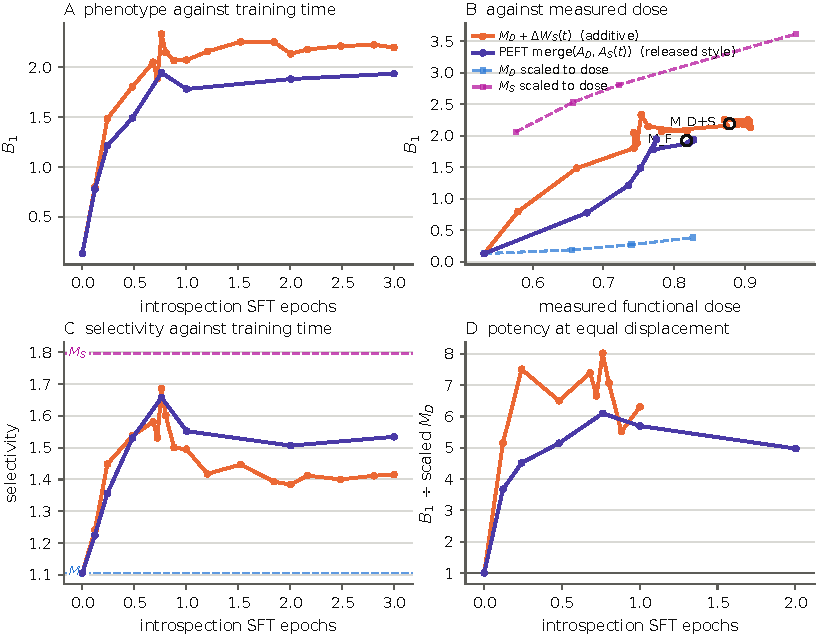
\includegraphics[width=0.95\linewidth]{figA_oct_sft_curve.pdf}
    \caption{The introspection SFT measured at 18 checkpoints through training (seed 123456, layer 15, forced prompt). The phenotype saturates well before one epoch, and the dose control shows this is not simply a matter of having moved the model further.\prov{workshop_iclr/figures/figA_oct_sft_curve.pdf}{scripts/appendix_oct/figA_oct_sft_curve.py}{workshop_iclr/data/figA_oct_sft_curve.csv}}
    \label{fig:oct-sft-curve}
\end{figure}





% \begin{figure}[!ht]
%     \centering
%     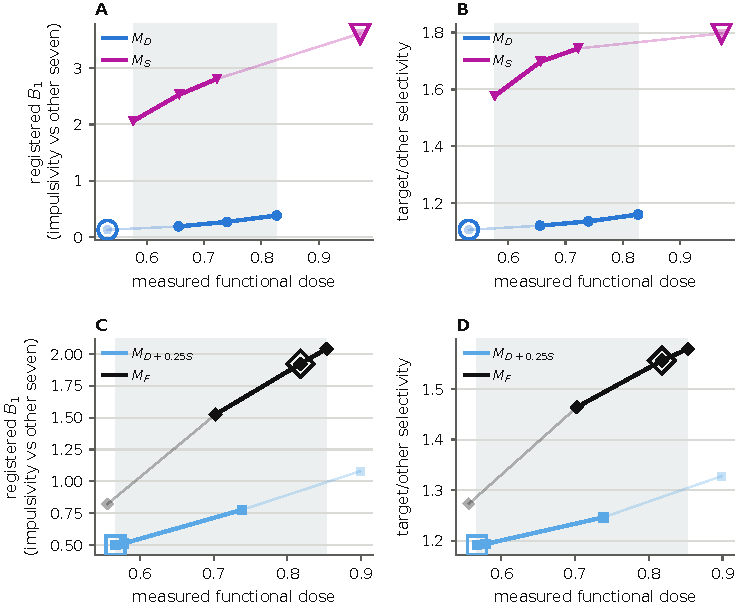
\includegraphics[width=0.75\linewidth]{figA_oct_matched_dose.pdf}
%     \caption{Stage comparisons at matched measured functional dose. \textbf{A,B} $M_D$ versus $M_S$; \textbf{C,D} $M_{D+0.25S}$ versus $M_F$, which differ only by peft's factor-space cross terms. Shading marks each pair's overlapping measured support, the only region in which the comparison is made; points outside it are drawn faint. Rings mark the trained $s{=}1$ state of each construction. Panel D reports selectivity rather than cosine because $M_F$'s trained state is itself the reference direction, so its cosine is pinned at $1.000$ by construction.\prov{workshop_iclr/figures/figA_oct_matched_dose.pdf}{scripts/appendix_oct/figA_oct_matched_dose.py}{workshop_iclr/data/figA_oct_matched_dose.csv}}
%     \label{fig:oct-matched-dose}
% \end{figure}


\paragraph{At matched functional dose, both stage differences survive.}
\begin{itemize}
    \item Each pair is compared only inside the range of measured dose where \emph{both} members were actually measured; nothing is extrapolated, and interpolation is restricted to each state's monotone prefix.
    \item $M_S$ against $M_D$: at matched dose $M_S$ exceeds $M_D$ on the registered endpoint by $8$--$13\times$ ($+2.12$ vs $+0.16$ at dose $0.586$, rising to $+3.11$ vs $+0.37$ at dose $0.817$), and is markedly more selective ($1.59$--$1.76$ against $1.11$--$1.16$).
    \item Reading: at comparable functional displacement, the DPO-generated introspection corpus learned through SFT is a far more potent carrier of the phenotype than the DPO weight update itself.
    \item What that does \emph{not} say: DPO is not shown to be unnecessary. DPO generated the corpus $M_S$ trains on, so removing DPO from the weights does not remove it from the causal history.
    \item Caveat bounding how strongly pair 1 can be phrased: reaching the overlap needs $M_D$ at $s\approx1.4$--$2.0$ and $M_S$ at $s\approx0.5$--$0.7$, so the comparison is between two scaled artifacts, neither of which is a trained state. This is inherent --- $M_D$ is simply the weakest perturbation.
\end{itemize}



\begin{table}[!ht]
\centering
\small
\begin{tabular}{llrrrrrl}
\toprule
target dose & state & scale & $B_1$ & $B_2$ & sel. & $k$ & source \\
\midrule
\multicolumn{8}{l}{\emph{$M_D$ vs $M_S$} -- overlap 0.576--0.827} \\
\midrule
0.586 & $M_D$ & 1.160 & +0.158 & +0.343 & 1.112 & 0.413 & interp \\
 & $M_S$ & 0.515 & +2.118 & +2.019 & 1.591 & 0.596 & interp \\
& \multicolumn{2}{r}{\emph{difference}} & \textbf{+1.960} & & \textbf{+0.479} & & \\
0.702 & $M_D$ & 1.523 & +0.236 & +0.436 & 1.129 & 0.342 & interp \\
 & $M_S$ & 0.647 & +2.721 & +2.598 & 1.730 & 0.527 & interp \\
& \multicolumn{2}{r}{\emph{difference}} & \textbf{+2.485} & & \textbf{+0.601} & & \\
0.817 & $M_D$ & 1.942 & +0.373 & +0.552 & 1.157 & 0.281 & interp \\
 & $M_S$ & 0.797 & +3.112 & +2.950 & 1.764 & 0.469 & interp \\
& \multicolumn{2}{r}{\emph{difference}} & \textbf{+2.739} & & \textbf{+0.607} & & \\
\midrule
\multicolumn{8}{l}{\emph{$M_{D+0.25S}$ vs $M_F$} -- overlap 0.567--0.853} \\
\midrule
0.578 & $M_{D+0.25S}$ & 1.025 & +0.513 & +0.632 & 1.193 & 0.438 & interp \\
 & $M_F$ & 0.561 & +0.927 & +1.018 & 1.302 & 0.467 & interp \\
& \multicolumn{2}{r}{\emph{difference}} & \textbf{+0.414} & & \textbf{+0.108} & & \\
0.710 & $M_{D+0.25S}$ & 1.382 & +0.729 & +0.843 & 1.237 & 0.363 & interp \\
 & $M_F$ & 0.814 & +1.551 & +1.598 & 1.470 & 0.381 & interp \\
& \multicolumn{2}{r}{\emph{difference}} & \textbf{+0.822} & & \textbf{+0.233} & & \\
0.842 & $M_{D+0.25S}$ & 1.787 & +0.972 & +1.062 & 1.299 & 0.306 & interp \\
 & $M_F$ & 1.042 & +2.004 & +2.026 & 1.572 & 0.323 & interp \\
& \multicolumn{2}{r}{\emph{difference}} & \textbf{+1.032} & & \textbf{+0.273} & & \\
\bottomrule
\end{tabular}
\caption{Stage comparisons at matched \emph{measured} functional dose (trait-vector displacement, layer 15, forced prompt, seed 123456). Anchors lie inside each pair's overlapping measured-dose support; \texttt{interp} marks a value interpolated between two measured rungs and \texttt{measured} one that a rung landed on. Nothing is extrapolated. \emph{difference} rows give the second state minus the first on $B_1$ and selectivity. Both contrasts that the raw decomposition suggested survive dose matching.}
\label{tab:oct-matched-dose}
\end{table}


\paragraph{The released merge is not the additive update it is read as.}
\begin{itemize}
    \item $M_F$ and $M_{D+0.25S}$ contain the same DPO and SFT components in the same $1{:}0.25$ proportion. They differ only in that peft combines LoRA \emph{factors}, which introduces the cross terms $B_D A_S + B_S A_D$.
    \item The cross terms are surplus rather than a mis-weighting, and this is derived rather than asserted. Extracting the factor coefficients from the released merge gives $A_{\mathrm{merged}}=\sqrt{2}A_D+(1/\sqrt{2})A_S$, and likewise for $B$. With the adapters' $\alpha/r=2$ and the merge's $\alpha/r=1$,
    \[\Delta W_{\mathrm{merged}}=\underbrace{2B_DA_D}_{=\;\Delta W_D}+\underbrace{0.5B_SA_S}_{=\;0.25\,\Delta W_S}+\underbrace{B_DA_S+B_SA_D}_{\text{artifact}}.\]
    \item So the two \emph{intended} terms come out at exactly the nominal $1.0$ and $0.25$: the merge does not mis-weight what OCT asked for, it adds structure OCT did not ask for.
    \item At matched dose those terms roughly double the behavioral contrast: $B_1$ goes from $+0.51$ to $+0.93$ at dose $0.578$, and from $+0.97$ to $+2.00$ at dose $0.842$ (Table~\ref{tab:oct-peft-merge}).
    \item This pair is the cleaner of the two: its overlap sits comfortably inside both states' measured ranges and contains both trained states.
    \item No share of behavior is attributed to the cross terms. Behavior is nonlinear in the weight update, so no such share is defined; the $61.9\%$ figure quoted elsewhere is a Frobenius norm ratio in weight space.
    \item Practical consequence: a reconstruction that merges DPO and SFT additively is not the same model as the released artifact, which matters for anyone comparing published OCT adapters against their own.
\end{itemize}

\begin{table}[!ht]
\centering
\small
\begin{tabular}{rrrrr}
\toprule
matched dose & $B_1$ without & $B_1$ with & sel. without & sel. with \\
 & cross terms & cross terms & cross terms & cross terms \\
\midrule
0.578 & +0.513 & \textbf{+0.927} & 1.193 & \textbf{1.302} \\
0.710 & +0.729 & \textbf{+1.551} & 1.237 & \textbf{1.470} \\
0.842 & +0.972 & \textbf{+2.004} & 1.299 & \textbf{1.572} \\
\bottomrule
\end{tabular}
\caption{The released-style merge is not the additive update it is often read as. peft's \texttt{add\_weighted\_adapter([DPO, SFT], [1, 0.25], \texttt{linear})} combines LoRA \emph{factors}, so $\Delta W_F = \Delta W_D + 0.25\,\Delta W_S + B_D A_S + B_S A_D$; $M_{D+0.25S}$ is the same construction with the two cross terms removed and is otherwise identical. At matched \emph{measured} functional dose, including the cross terms changes $B_1$ from $+0.51$ to $+0.93$ at dose $0.578$ and from $+0.97$ to $+2.00$ at dose $0.842$. We do not report a share of behaviour attributable to the cross terms: behaviour is nonlinear in the weight update, so no such share is defined. (The $61.9\%$ figure quoted elsewhere is a Frobenius norm ratio in weight space, not a behavioural one.)}
\label{tab:oct-peft-merge}
\end{table}


\paragraph{The phenotype is installed well before one epoch of SFT.}
18 SFT checkpoints were measured to identify when during training the phenotype arrives (Fig.~\ref{fig:oct-sft-curve}, Table~\ref{tab:oct-sft-curve}). As discussed in \ref{sec:results-sft}, $82\%$ of the final $B_1$ is present by $0.48$ epochs, with curve flattening from roughly $0.68$ epochs onward. This effect survives control for functional effect (dose). $B_1$ and selectivity peak at 0.76 epoch, but the reliability and reason for this apparent behavior hasn't been investigated further.

\paragraph{Two apparent trends on the curve that did not survive denser sampling.}
\begin{itemize}
    \item An apparent overshoot did not survive denser sampling. A sparse curve showed a peak at $0.76$ epochs and a dip at $1.00$ with \emph{disjoint question-bootstrap intervals}. Four extra checkpoints show adjacent ones, 15 optimizer steps apart, move $B_1$ by up to $0.446$, against a plateau sd of $0.129$; the $0.76$ value sits $1.7$ sd above the plateau mean, unremarkable for eight samples.
    \item The intervals were correct and irrelevant. They measure variance over evaluation questions, not over checkpoints, and the relevant variance is the larger one. An interval that answers a question you did not ask still looks decisive.
    \item An apparent \emph{decline} in selectivity past one epoch is likewise \textbf{not established}. Judged against checkpoint scatter rather than a question bootstrap, over nine checkpoints from $1.0$ to $3.0$ epochs the slope is $-0.028$ selectivity per epoch (SE $0.015$, $1.8$ SE from zero) against a threshold of $2$ SE fixed before the numbers existed.
    \item Dose-controlling it does not rescue the decline either, and here the control is available: all nine late checkpoints sit inside $M_D$'s measured ladder ($0.531$--$0.972$), so nothing is extrapolated. The excess over $M_D$ at matched dose slopes at $-0.041$ per epoch (SE $0.020$, $2.1$ SE), which would cross the threshold --- but leave-one-out refits span $-2.3$ to $-0.9$ SE, so the result rests on one point rather than on the trend.
    \item That point is the $1.00$-epoch checkpoint, which sits $5.2$ sd from the other eight and at a markedly lower dose ($0.782$ against $0.87$--$0.91$). Excluding it, the remaining eight checkpoints from $1.20$ to $3.00$ epochs have excess $+0.229$ with sd $0.023$.
    \item So the positive statement is available and is the one worth making: past roughly $1.2$ epochs specificity \emph{settles and stays put} rather than progressively eroding. Training past one epoch keeps displacing the model without making the shift either more or less trait-specific.
    \item This is the second time in this work that a trend read off sparse checkpoints evaporated once the sampling was made dense.
\end{itemize}


\begin{table}[!ht]
\centering
\footnotesize
\setlength{\tabcolsep}{4pt}
\begin{tabular}{lrrrrrrl}
\toprule
construction & step & epoch & dose & $B_1$ & sel. & $k$ & vs $M_D$ \\
\midrule
\multicolumn{8}{l}{\emph{$M_D{+}\Delta W_S$}} \\
$M_D$ (no SFT) & 0 & 0.000 & 0.531 & +0.132 & 1.106 & 0.448 & 1.0$\times$ \\
$M_D{+}\Delta W_S$ & 45 & 0.120 & 0.579 & +0.798 & 1.241 & 0.445 & 5.2$\times$ \\
$M_D{+}\Delta W_S$ & 90 & 0.240 & 0.662 & +1.484 & 1.448 & 0.405 & 7.5$\times$ \\
$M_D{+}\Delta W_S$ & 180 & 0.481 & 0.743 & +1.804 & 1.537 & 0.382 & 6.5$\times$ \\
$M_D{+}\Delta W_S$ & 255 & 0.681 & 0.743 & +2.049 & 1.581 & 0.397 & 7.4$\times$ \\
$M_D{+}\Delta W_S$ & 270 & 0.722 & 0.748 & +1.887 & 1.531 & 0.380 & 6.7$\times$ \\
$M_D{+}\Delta W_S$ & 285 & 0.762 & 0.754 & +2.333 & 1.686 & 0.399 & 8.0$\times$ \\
$M_D{+}\Delta W_S$ & 300 & 0.802 & 0.764 & +2.146 & 1.602 & 0.378 & 7.1$\times$ \\
$M_D{+}\Delta W_S$ & 330 & 0.882 & 0.818 & +2.067 & 1.500 & 0.363 & 5.5$\times$ \\
$M_D{+}\Delta W_S$ & 375 & 1.002 & 0.782 & +2.071 & 1.495 & 0.374 & 6.3$\times$ \\
$M_D{+}\Delta W_S$ & 450 & 1.203 & 0.874 & +2.157 & 1.418 & 0.393 & \textit{n/a} \\
$M_D{+}\Delta W_S$ & 570 & 1.523 & 0.871 & +2.254 & 1.447 & 0.404 & \textit{n/a} \\
$M_D{+}\Delta W_S$ & 690 & 1.844 & 0.905 & +2.252 & 1.393 & 0.394 & \textit{n/a} \\
$M_D{+}\Delta W_S$ & 750 & 2.004 & 0.908 & +2.134 & 1.384 & 0.385 & \textit{n/a} \\
$M_D{+}\Delta W_S$ & 810 & 2.165 & 0.890 & +2.177 & 1.412 & 0.393 & \textit{n/a} \\
$M_D{+}\Delta W_S$ & 930 & 2.485 & 0.904 & +2.211 & 1.400 & 0.387 & \textit{n/a} \\
$M_D{+}\Delta W_S$ & 1050 & 2.806 & 0.907 & +2.224 & 1.412 & 0.391 & \textit{n/a} \\
$M_D{+}\Delta W_S$ & 1122 & 2.998 & 0.903 & +2.197 & 1.415 & 0.388 & \textit{n/a} \\
\midrule
\multicolumn{8}{l}{\emph{merge}} \\
$M_D$ (no SFT) & 0 & 0.000 & 0.531 & +0.132 & 1.106 & 0.448 & 1.0$\times$ \\
merge & 45 & 0.120 & 0.677 & +0.778 & 1.225 & 0.363 & 3.7$\times$ \\
merge & 90 & 0.240 & 0.735 & +1.214 & 1.356 & 0.343 & 4.5$\times$ \\
merge & 180 & 0.481 & 0.753 & +1.490 & 1.530 & 0.318 & 5.1$\times$ \\
merge & 285 & 0.762 & 0.775 & +1.943 & 1.658 & 0.338 & 6.1$\times$ \\
merge & 375 & 1.002 & 0.770 & +1.781 & 1.552 & 0.324 & 5.7$\times$ \\
merge & 750 & 2.004 & 0.821 & +1.881 & 1.506 & 0.328 & 5.0$\times$ \\
merge & 1122 & 2.998 & 0.828 & +1.935 & 1.534 & 0.331 & \textit{n/a} \\
\bottomrule
\end{tabular}
\caption{The introspection SFT measured at checkpoints through training (seed 123456, layer 15, forced prompt). \emph{step} is optimizer steps; one epoch is 374.2 steps, so the run is 1122 steps and the final row is the trained endpoint. \emph{dose} is \emph{measured} functional dose, never weight norm. The last column is the dose control: $B_1$ divided by $B_1$ of $M_D$ scaled to the same measured dose, so $1.0\times$ would mean the checkpoint is worth no more than moving the model that far with the DPO adapter alone. Nothing is extrapolated outside $M_D$'s measured range. The two constructions differ in SFT weight ($1.00$ against $0.25$) as well as in the merge, so the gap between them is not the cross-term contribution.}
\label{tab:oct-sft-curve}
\end{table}


\begin{figure}[!ht]
    \centering
    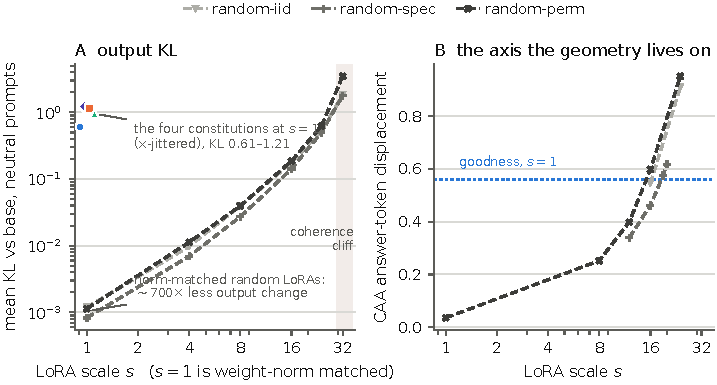
\includegraphics[width=0.95\linewidth]{figA1_dose_calibration.pdf}
    \caption{Three different dose axes --- weight norm, output KL, and CAA answer-token displacement --- do not agree, which is why every matched comparison in this paper is sited by measurement rather than by nominal LoRA scale. At $s{=}1$ a norm-matched untrained LoRA is effectively inert (neutral-prompt KL $\sim\!500$--$700\times$ below a trained adapter). Panel A is also what bounds the untrained arms: the rungs used ($s = 16$--$19$) sit within roughly a factor of two of the point where KL climbs steeply.\prov{workshop_iclr/figures/figA1_dose_calibration.pdf}{workshop_iclr/scripts/figA1_dose_calibration.py}{workshop_iclr/data/figA1_dose_calibration.csv}}
    \label{fig:dose-calibration}
\end{figure}

\section{Definitions and Estimator Notes}
\label{app:definitions}

Every quantity used anywhere in the paper is collected in Table~\ref{tab:symbols}, in the
order the paper introduces it. Indices are $c$ (constitution or intervention arm), $t$
(trait, $T=8$), $p$ (persona, $P=10$), and $q$ (CAA question); all geometric quantities are
at layer $\ell\in\{15,20\}$ and default to $\ell=15$ where unstated.

{\footnotesize
\begin{longtable}{@{}p{0.20\textwidth}p{0.40\textwidth}p{0.34\textwidth}@{}}
\caption{Symbols, estimators and the exact form of every statistic reported.}
\label{tab:symbols}\\
\toprule
\textbf{Symbol} & \textbf{Definition} & \textbf{Notes} \\
\midrule
\endfirsthead
\multicolumn{3}{@{}l}{\emph{Table~\ref{tab:symbols}, continued}}\\
\toprule
\textbf{Symbol} & \textbf{Definition} & \textbf{Notes} \\
\midrule
\endhead
\bottomrule
\endfoot

\multicolumn{3}{@{}l}{\emph{Objects}}\\[2pt]
$V_{c,t,p}$ & $\in\mathbb{R}^{4096}$; CAA trait vector, contrastive-pair activation difference at the answer token & Base model written $V_{\mathrm{base},t,p}$ \\[4pt]
$dV_{c,t,p}$ & $V_{c,t,p}-V_{\mathrm{base},t,p}$ & Adapter-induced change; the object every statistic below is built from \\[4pt]
$\bar V_{c,t}$ & $\tfrac{1}{P}\sum_{p}V_{c,t,p}$ & Persona centroid within a (constitution, trait) cell \\
\midrule

\multicolumn{3}{@{}l}{\emph{Factorial decomposition (Eq.~\ref{eq:decomp})}}\\[2pt]
$\mu,C_c,T_t,P_p$ & Grand, constitution, trait and persona main effects in $dV_{c,t,p}=\mu+C_c+T_t+P_p+(CT)_{c,t}+(CP)_{c,p}+(TP)_{t,p}+(CTP)_{c,t,p}$ & ANOVA-style; $P_p$ the persona \emph{term}, $P=10$ the persona \emph{count} \\[4pt]
$(CTP)_{c,t,p}$ & Residual triple interaction, after all lower-order terms are removed & The registered quantity; $3.6\%$ of trained squared change at L15 \\[4pt]
Term share & Squared norm of a term over total squared change, summing to $1$ across the eight terms & Reported in Fig.~\ref{fig:ctp}A \\
\midrule

\multicolumn{3}{@{}l}{\emph{Persona-common structure}}\\[2pt]
$dG_{c,t}$ & $\tfrac{1}{P}\sum_{p}dV_{c,t,p}$ & Persona-common shift \\[4pt]
Partition identity & $\mathrm{mean}_p\|dV_{c,t,p}\|^2=\|dG_{c,t}\|^2+\mathrm{mean}_p\|dV_{c,t,p}-dG_{c,t}\|^2$ & Exact, not a fit: the cross term vanishes because $dG$ is the mean \\[4pt]
Common-shift share & $\|dG_{c,t}\|^2\big/\mathrm{mean}_p\|dV_{c,t,p}\|^2$ & Bounded in $[0,1]$ by construction; $67$--$77\%$ at L15 \\[4pt]
Relative common shift & $\|dG_{c,t}\|\big/\mathrm{mean}_p\|V_{\mathrm{base},t,p}\|$ & Fig.~\ref{fig:trait-selectivity}B; a magnitude, never a direction or valence \\[4pt]
Trait selectivity & Ratio of the relative common shift averaged over the target traits to the same averaged over the remaining traits & Targets are \texttt{impulsivity} (registered) and \texttt{risk\_taking} (added post hoc by the geometry) \\
\midrule

\multicolumn{3}{@{}l}{\emph{Persona geometry}}\\[2pt]
$D_{c,t}$ & $\tfrac{1}{P}\sum_{p}\|V_{c,t,p}-\bar V_{c,t}\|^2$ & Dispersion; plotted as the RMS ratio $\sqrt{D_{c,t}/D_{\mathrm{base},t}}$ \\[4pt]
$R_{c,t}$ & $\in\mathbb{R}^{45}$, entries $\|V_{c,t,p}-V_{c,t,q}\|^2$ for $p<q$ & RDM. Euclidean distance is invariant to adding a common vector, so the large shared shift cancels exactly \\[4pt]
RDM preservation & $\rho=\mathrm{Spearman}\big(R_{c,t},R_{\mathrm{base},t}\big)$ over the 45 pairs & $\rho=1$ means relative persona ordering is untouched \\[4pt]
Attenuation correction & $\rho\big/\sqrt{\mathrm{rel}_{c}\cdot\mathrm{rel}_{\mathrm{base}}}$ & Corrected and raw values are never mixed within a panel \\
\midrule

\multicolumn{3}{@{}l}{\emph{Dose}}\\[2pt]
$s$ & LoRA application scale, as passed to the adapter & \emph{Not} a dose: at $s{=}1$ the arms span measured dose $0.54$--$1.11$ \\[4pt]
Trait-vector displacement & $\|V_{c,t,p}-V_{\mathrm{base},t,p}\|\big/\|V_{\mathrm{base},t,p}\|$, averaged over cells & Measured on the same cached activations the geometry uses \\[4pt]
Functional dose & Trait-vector displacement normalised so \texttt{goodness} at $s{=}1$ equals $1.0$ & The only admissible $x$-axis for a matched comparison; $\|\Delta W\|_F$ is a diagnostic column, never dose \\
\midrule

\multicolumn{3}{@{}l}{\emph{Global linear reshaping}}\\[2pt]
$X_{t,p},\,Y_{c,t,p}$ & $V^{\mathrm{base}}_{t,p}-\bar V^{\mathrm{base}}_{t}$ and $V_{c,t,p}-\bar V_{c,t}$ & Persona-centred, so the common shift is removed before fitting \\[4pt]
$\hat A_c$ & $\arg\min_A\sum_{(t,p)\in\mathrm{train}}\|Y_{c,t,p}-AX_{t,p}\|^2$ & One reduced-rank map per arm, shared across all trait$\times$persona cells \\[4pt]
Fraction removed & Squared error removed by $\hat A_c$ on held-out cells & $39$--$54\%$ trained; the orthogonal (Procrustes) restriction explains less \\
\midrule

\multicolumn{3}{@{}l}{\emph{Behavioral preference}}\\[2pt]
Log-odds & $\log$ odds of the trait-positive over the trait-negative answer letter, per (persona, question) & Forced-choice CAA items; no completion is generated \\[4pt]
$a,\,k$ & OLS fit $\mathrm{logodds}^{\mathrm{arm}}=a+k\,\mathrm{logodds}^{\mathrm{base}}$ & $a$ is the compression-corrected preference at base indifference; $k$ is retention \\[4pt]
Naive delta & $\mathrm{mean}(\mathrm{logodds}^{\mathrm{arm}}-\mathrm{logodds}^{\mathrm{base}})$ & Reported for contrast only. Invalid: it mirrors the base model's own preferences wherever $k$ is small \\[4pt]
$B_1,\,B_2$ & $a$ on \texttt{impulsivity} minus mean $a$ over the other seven traits; $B_2$ additionally treats \texttt{risk\_taking} as a target & $B_1$ is the registered endpoint \\
\midrule

\multicolumn{3}{@{}l}{\emph{Estimators}}\\[2pt]
Cross-fitting & $\mathbb{E}[(\hat\theta^{A})^\top\hat\theta^{B}]=\|\theta\|_2^2$ for disjoint samples $A,B$, replacing the biased $\|\hat\theta\|_2^2$ & Derived in \S\ref{app:anova}, with the split used here (500 questions, 40 repetitions of disjoint 250-question batches) \\[4pt]
Question bootstrap & $95\%$ intervals, 200 replicates, draws shared across arms & Paired, so arm-to-arm comparisons are valid. Conditions on these 8 traits and 10 personas: not population inference, and not uncertainty over training seeds \\
\end{longtable}
}

\section*{Reproducibility Statement}
\label{sec:repro}
\begin{itemize}
    \item All figure paths quoted in the captions are relative to the code release at \url{\provbase}.
    \item Every figure caption names the script that draws it and a CSV of the exact values it plots. Those CSVs are written by the same scripts from cached analysis outputs under \path{outputs/analysis/}, so every number in every figure is auditable without rerunning inference.
    \item No figure in this paper requires a forward pass to rebuild. The whole set is CPU-reproducible from the archived analysis outputs.
    \item Arm names, ordering, color and marker come from a single style module; the palette is validated against Machado color-vision-deficiency transforms rather than asserted.
    \item \textbf{TODO.} Add exact adapter identifiers, the extraction scripts and their environment pins, the random-control constructors, the bootstrap and cross-fitting code, and the preregistration.
\end{itemize}

\paragraph{The published pipeline no longer describes the published adapters.}
\begin{itemize}
    \item Reproducing OCT from the repository at HEAD trains the introspection stage for one epoch. The released adapters were trained for three.
    \item The commit that changed it (\texttt{bd20b87}, ``introspection 1 epoch instead of 3'') lands \textbf{8 minutes 23 seconds after} the final upload of the released artifacts. Checked at both candidate release dates, the introspection runner reads \texttt{--max\_epochs 3}.
    \item The DPO stage is unaffected: that runner has not changed since before the release and is byte-equivalent on every value used.
    \item Worth recording because of how it was caught. Every \emph{behavioral} gate criterion passed the wrong artifact; the only check that failed it was a weight-norm comparison. A reproduction validated on behavior alone would have proceeded on a model trained for a third as long as the one it was reproducing.
\end{itemize}


\end{document}
